\subsubsection{VLAN de~\nameref{itm:vlan20}}
\par Habiendo ya pasado por el proceso de analizar una VLAN, nos encontramos en una
situaci\'on mucho m\'as concisa. En esta VLAN esperamos encontrar mucho menos tr\'afico
que en la anterior. Este razonamiento se debe a que esta es una red de servidores, con
lo cual se espera estar tomando datos de un ambiente mucho m\'as administrado, con
menos varianza de las terminales que se prenden/apaguan conectan/desconectan.

\par Estas caracter\'isticas del entorno nos hacen razonar tambi\'en que al ser
servidores con mucha menos manipulaci\'on, con las conexiones dentro de la LAN
seguramente mucho m\'as estables ya que nadie est\'a usando est\'as terminales
para \textit{salir} a internet o utilizandolas activamente con servicios que
deban salir a otra red salvo para la comunicaci\'on con los usuarios que se conectan
a los mismos.

\par As\'i pues, pasamos a los datos concretos de nuestro an\'alisis:

\begin{table}[!h]
\centering
  \begin{tabular}{c c}
    Fuente de Datos & Entrop\'ia \\
    \hline\hline
    Direcci\'on Origen & 3.01743 \\
    Direcci\'on Destino & 5.71059 \\
    \hline\hline
    \#IPs de las Fuentes & 2051\\
    \#Paquetes Capturados & 874806\\
    \hline
    \end{tabular}
  \bigskip
  \caption{Entrop\'ia VLAN \nameref{itm:vlan20}}
  \label{tab:vlan20_entropia}
\end{table}

\par Curiosamente, los resultados aqu\'i obtenidos nos dan una cantidad de paquetes
similar a la de la VLAN \nameref{itm:vlan10}. Compararemos estos resultados m\'as
adelante en la secci\'on \ref{sec:escenario1_supl}.


\subsubsection*{\underline{VLAN \nameref{itm:vlan20}: Fuente Origen}}\label{subsubsec:vlan20_src}
\par Pasamos ahora a visualizar las distintas probabilidades que nos d\'a esta fuente de
datos.

\begin{figure}[!ht]
    \centering
    \includegraphics[width=0.5\textwidth]{escenario_1/vlan20/vlan20_src_bars_percentile90}
    \caption{Probabilidades VLAN \nameref{itm:vlan20} - Fuente Origen}
    \label{fig:vlan20_src_prob_per90}
\end{figure}

\par El resultado inmediato que se puede observar aqu\'i es la poca cantidad de IPs
requeridas para componer el percentil 90. Se ver\'a m\'as adelante que la concentraci\'on
de la informaci\'on en esta VLAN es mucho mayor que en el caso anterior. Se puede
ver con claridad que con tan solo con las 5 IPs de mayor probabilidad muestral se obtiene
la probabilidad acumulada del 90\% de la fuente. A\'un as\'i, vale la pena mencionar
nuevamente el dato expresado en la tabla \ref{tab:vlan20_entropia}, donde se puede
observar que la cantidad de IPs/S\'imbolos que nos di\'o la fuente fue extensamente
mayor.

\par Esto ya parecer\'ia estar indicando que en la red hay muy pocas terminales que
env\'ian paquetes ARP, al menos con una frecuencia comparable al caso de la VLAN
ya analizada.


\subsubsection*{\underline{VLAN \nameref{itm:vlan20}: Fuente Destino}}\label{subsubsec:vlan20_dst}
\par Veamos ahora que pasa con las otras terminales a la hora de responder a los
paquetes ARP. La pregunta que nos realizamos es si esas 5 terminales que acaparaban
todo el tr\'afico de env\'io de paquetes ARP es entre ellas, distribu\'ido entre
las dem\'as direcciones de la LAN o si simplemente son paquetes ARP env\'iados para
monitorear la red, en cuyo caso ir\'ian dirigidos a IPs inexistentes.

\begin{figure}[!ht]
    \centering
    \includegraphics[width=0.5\textwidth]{escenario_1/vlan20/vlan20_dst_bars_percentile90}
    \caption{Probabilidades VLAN \nameref{itm:vlan20} - Fuente Destino}
    \label{fig:vlan20_dst_prob_per90}
\end{figure}

\par Notoriamente en este caso se puede observar como para alcanzar el percentil
90 se necesitan de algo menos que las 1200 direcciones IPs con mayor probabilidad
muestral. Ya esto nos da la pauta, a diferencia de lo que ve\'iamos observando
hasta este momento, de que en este entorno la fuente de direcciones destino
no est\'a tan concentrada. De hecho, parecer\'ia haber una \'unica IP que
es destinatario de m\'as de alg\'un paquete ARP, dandonos a entender que no es
una coincidencia impulsada, quiz\'as, por el tama\~no de la red el hecho de que
sea la \'unica IP de esta fuente de datos con una probabilidad no desestimable.

\begin{figure}[!ht]
    \centering
    \includegraphics[width=0.5\textwidth]{escenario_1/vlan20/vlan20_dst_probabilities_with_labels}
    \caption{IPs VLAN \nameref{itm:vlan20} - Fuente Destino}
    \label{fig:vlan20_dst_prob_ips}
\end{figure}


\par Ya llegados a estas instancias, nos resulta interesante ver la siguiente tabla
y como contrasta con la del caso anterior:

\begin{table}[!h]
\centering
  \begin{tabular}{c c c c}
    Fuente& 
    Entrop\'ia & \begin{tabular}{@{}c@{}}Concentraci\'on \\ Percentil 90\end{tabular} 
    & \begin{tabular}{@{}c@{}}Concentraci\'on \\ Percentil 80\end{tabular}\\
    \hline\hline
    Origen & 3.01743 & 0.0024\% & 0.0014\%\\
    Destino & 5.71059 & 0.573\% & 0.183\%\\
    \hline\hline
    \end{tabular}
  \bigskip
  \caption{Concentraci\'on VLAN \nameref{itm:vlan10}}
  \label{tab:vlan20_concentracion}
\end{table}

\par Los n\'umeros aqu\'i ya nos est\'an diciendo mucho sobre la red. La baja entro\'ia
de la fuente de origen nos comunica que estamos ante una fuente de datos bastante
predecible. De hecho, esto luego se ve confirmado por la baja concentraci\'on de 
s\'imbolos que componen el percentil 90 y 80. Claramente con muy pocas direcciones
ya se tiene una gran probabilidad acumulada de la fuente, sabiendo entonces que seguramente,
si hay un paquete ARP, poder indicar 6 direcciones sobre 2051 con una probabilidad muestral
del 90\%.

\par Por lo contrar\'io, la fuente destino es ya bastante m\'as impredecible. Si bien su
entrop\'ia no es alta (al menos comparada con los otros casos ya expuestos), vemos una
concentraci\'on considerable (respecto de la fuente de origen) en el percentil 90. Pero
observando la figura \ref{fig:vlan20_dst_prob_ips}, podemos ver que en realidad, hay
una direcci\'on particular que tiene casi un 25\% de probabilida de surgir de esta fuente, pero
ocurre que todas las dem\'as direcciones tienen una probabilidad muy baja. Por lo tanto,
sabemos que existe una \'unica IP en realidad que podr\'ia llegar a ser esperada con cierta
justificaci\'on, pero es todo lo que podemos decir de este dominio de colisi\'on.


\subsubsection*{\underline{VLAN \nameref{itm:vlan20}: Ambas Fuentes}}\label{subsubsec:vlan20_src_dst}
\par A diferencia de la VLAN de \nameref{itm:vlan10}, aqu\'i ya pudimos obtener varios
resultados interesantes y bastante expl\'icitos sobre el comportamiento de las fuentes
de informaci\'on analizados. No obstante, es interesante verificar como se compone
el gr\'afo de esta fuente, en parte para confirmar las hip\'otesis planteadas sobre
el funcionamiento de la red y tambi\'en para verificar si no hay alg\'un dato
o caractar\'istica que no pueda ser visto mediante las probabilidades ya expuestas.

\par En el grafo que se presenta a continuaci\'on se utilizan las mismas reglas de coloreo
y de grosores ya explicadas en la secci\'on \ref{subsubsec:vlan10_src_dst}. Al igual
que en el caso anterior, desestimamos aquellos ejes que no tuvieran un peso
superior a 70 (en lugar de 500 del caso anterior, ya que esta VLAN contiene muchas
menos direcciones IP y mucho menos tr\'afico ARP tambi\'en). La justificaci\'on subyacente
es la misma que antes: luego de 77 horas de captura de paquetes, si un servidor
trata de obtener espor\'adicamente la \textit{MAC} de otra terminal, es un dato
que no nos suma a la topolog\'ia que tratamos de descubrir (ya que agregar\'a ejes
que ocurren con muy poca probabilidad).

\begin{figure*}[!t]
    \centering
    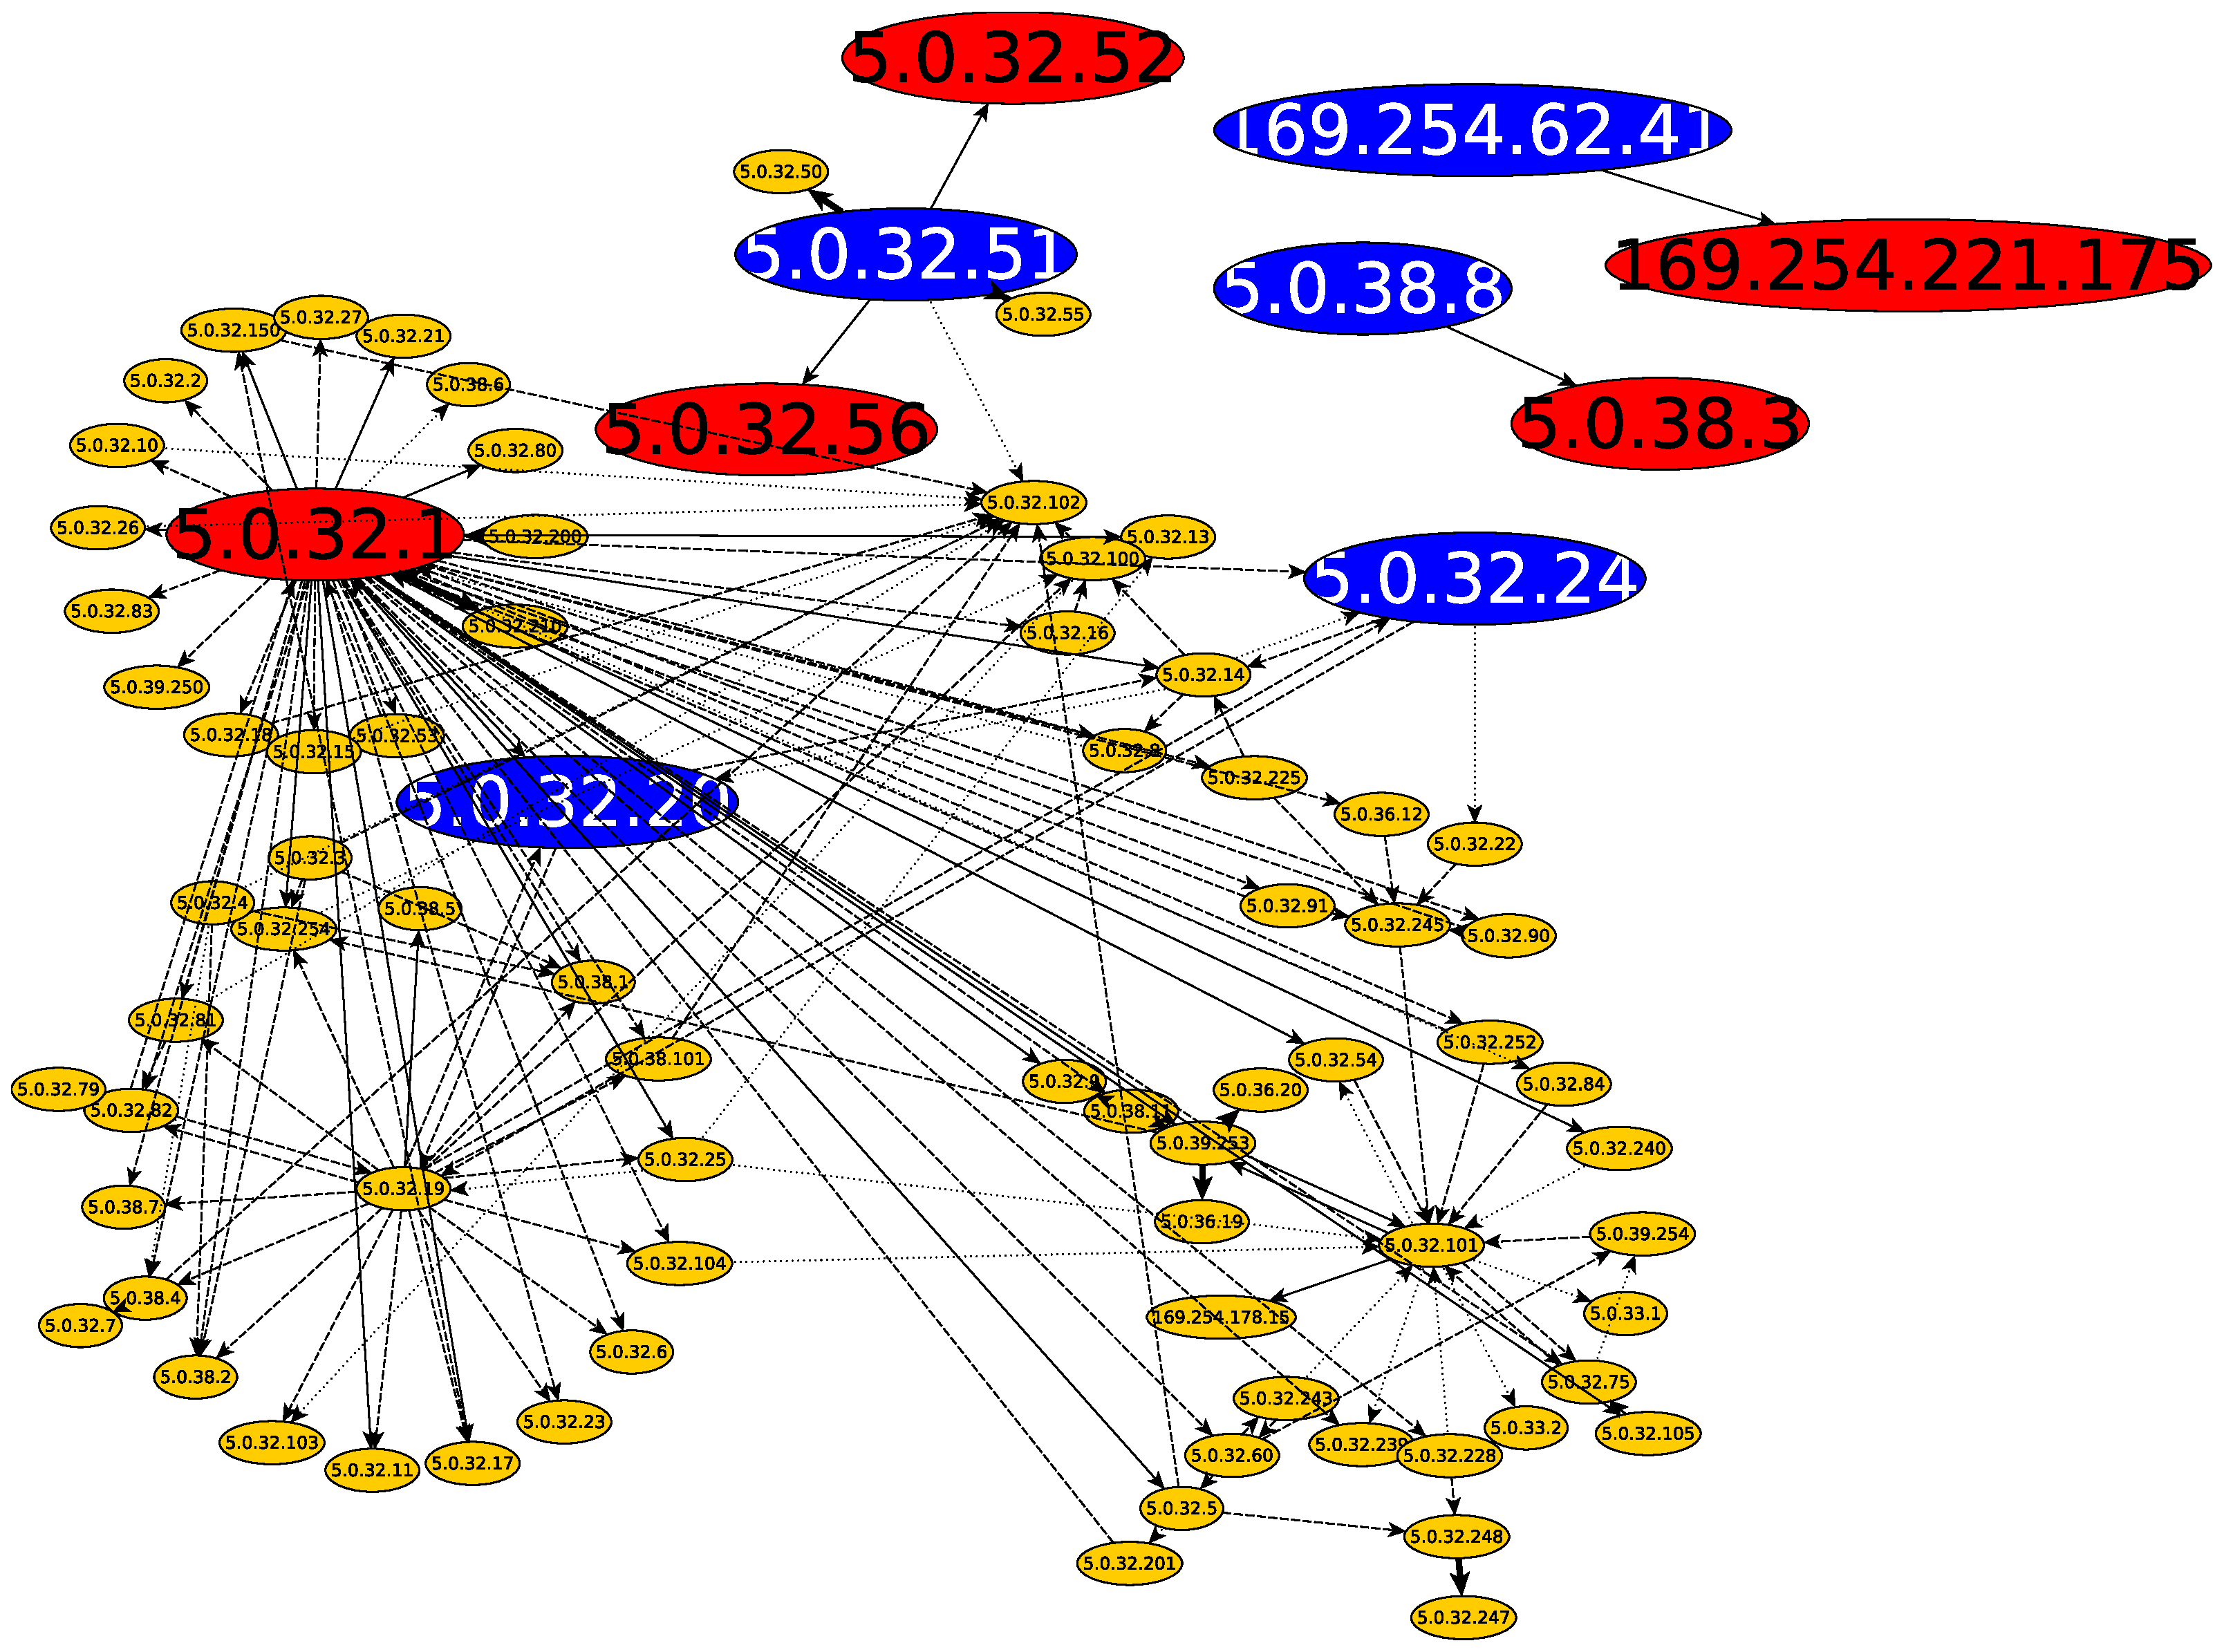
\includegraphics[width=\textwidth]{img/graph/escenario_1/vlan20/vlan20_70toEnd}
    \caption{Grafo VLAN \nameref{itm:vlan20}}
    \label{fig:vlan20_grafo}
\end{figure*}

\par En la figura \ref{fig:vlan20_grafo} se pueden observar ciertas cosas esperables
como otras que no tanto.

\par En primer lugar, salvo los nodos inclu\'idos en los percentiles 90, no pareciese
haber pedidos de resoluci\'on de \textit{MAC}\footnote{Abuso de notaci\'on.} entre
los hosts con poca probabilidad. Como posibles excepciones a esto se pueden ver las
IPs \textit{5.0.32.101, 5.0.32.19 y 5.0.32.102}. Si bien hay algunas otras con menor
afluencia que estas tres, hay que mencionar que ya en estas direcciones que mencionamos,
los ejes est\'an representados con flechas punteadas (es decir, no hay un pedido realmente
consistente de la \textit{MAC} de estos hosts).

\par Siguiendo con esta l\'inea de razonamiento, podemos ver que los ejes que denotan
"conexiones" consistentes entre servidores son pocos (lo cual es coherente con la
informaci\'on analizada hasta aqu\'i). Destacan por ah\'i algunas relaciones entre
la IP \textit{5.0.32.1}, claramente consultada por casi todos los nodos de la red (%
lo cual nos lleva a intu\'ir que este es un nodo importante de la red, ya que casi
todos en alg\'un momento durante la semana requieren poder conectarse a \'el) y 
los pedidos constantes de la \textit{5.0.32.51} para las direcciones \textit{5.0.32.56,
5.0.32.52, 5.0.32.50 y 5.0.32.55}\footnote{Estas \'ultimas dos ni siquiera forman
parte de uno de los percentiles 90}. Claramente aqu\'i, si consideramos que la
\textit{5.0.32.1} es posiblemente el \textit{gateway} de la red, nos encontramos
con 4 interfases de red que trabajan constantemente codo a codo (lo cual tambi\'en
explicar\'ia lo cercano de sus direcciones, aunque esto es simplemente algo que
se suele hacer en los \'ambitos de administraci\'on de servidores\footnote{Y \'unicamente
cuando los servidores son reci\'en instalados y hay IPs libres en la red.}).

\par Notoriamente, un resultado que no esper\'abamos encontrar es ver que parece
ser la \textit{5.0.32.1} el gateway de la red en lugar de la \textit{5.0.38.3} o la
\textit{5.0.38.8}, que son las direcciones con mayor probabilidad en ambas fuentes de informaci\'on.
Esto sorprende, pero como se ha dicho anteriormente, estando en una red de servidores no se espera
que estos deban de comunicarse con otras redes tan seguido como por ah\'i lo hacen
las terminales de otras redes (principalmeente porque los servidores se comunican
entre s\'i para la gran parte de sus tareas\footnote{Los servidores una vez instalados
no se actualizan jam\'as. \textit{If ain't broken, don't fix it}. Manual b\'asico
del administrador de servidores.}).

\par Prosiguiendo, se nota que el tr\'afico entre la \textit{5.0.38.8} hacia
la \textit{5.0.38.3} es constante, ya que esta \'ultima tiene la probabilidad
m\'as alta de la fuente de destino y la primera la tiene en la fuente de origen. Claramente
estas dos terminales deben estar proveyendo alg\'un tipo de servicio, o utilizando
una el servicio de la otra, constantemente, ya que sus probabilidades son
notoriamente mayores que la del resto de las IPs.

\subsubsection*{\underline{VLAN \nameref{itm:vlan20}: Conclusiones}}\label{subsubsec:vlan20_conclusiones}
